\documentclass[twoside]{article}

% Packages required by doxygen
\usepackage{fixltx2e}
\usepackage{calc}
\usepackage{doxygen}
\usepackage[export]{adjustbox} % also loads graphicx
\usepackage{graphicx}
\usepackage[utf8]{inputenc}
\usepackage{makeidx}
\usepackage{multicol}
\usepackage{multirow}
\PassOptionsToPackage{warn}{textcomp}
\usepackage{textcomp}
\usepackage[nointegrals]{wasysym}
\usepackage[table]{xcolor}

% Font selection
\usepackage[T1]{fontenc}
\usepackage[scaled=.90]{helvet}
\usepackage{courier}
\usepackage{amssymb}
\usepackage{sectsty}
\renewcommand{\familydefault}{\sfdefault}
\allsectionsfont{%
  \fontseries{bc}\selectfont%
  \color{darkgray}%
}
\renewcommand{\DoxyLabelFont}{%
  \fontseries{bc}\selectfont%
  \color{darkgray}%
}
\newcommand{\+}{\discretionary{\mbox{\scriptsize$\hookleftarrow$}}{}{}}

% Page & text layout
\usepackage[screen,margin=0.5in]{geometry}
\tolerance=750
\hfuzz=15pt
\hbadness=750
\setlength{\emergencystretch}{15pt}
\setlength{\parindent}{0cm}
\setlength{\parskip}{3ex plus 2ex minus 2ex}
\makeatletter
\renewcommand{\paragraph}{%
  \@startsection{paragraph}{4}{0ex}{-1.0ex}{1.0ex}{%
    \normalfont\normalsize\bfseries\SS@parafont%
  }%
}
\renewcommand{\subparagraph}{%
  \@startsection{subparagraph}{5}{0ex}{-1.0ex}{1.0ex}{%
    \normalfont\normalsize\bfseries\SS@subparafont%
  }%
}
\makeatother

% Headers & footers
\usepackage{fancyhdr}
\pagestyle{fancyplain}
\fancyhead[LE]{\fancyplain{}{\bfseries\thepage}}
\fancyhead[CE]{\fancyplain{}{}}
\fancyhead[RE]{\fancyplain{}{\bfseries\leftmark}}
\fancyhead[LO]{\fancyplain{}{\bfseries\rightmark}}
\fancyhead[CO]{\fancyplain{}{}}
\fancyhead[RO]{\fancyplain{}{\bfseries\thepage}}
\fancyfoot[LE]{\fancyplain{}{}}
\fancyfoot[CE]{\fancyplain{}{}}
\fancyfoot[RE]{\fancyplain{}{\bfseries\scriptsize Generated by Doxygen }}
\fancyfoot[LO]{\fancyplain{}{\bfseries\scriptsize Generated by Doxygen }}
\fancyfoot[CO]{\fancyplain{}{}}
\fancyfoot[RO]{\fancyplain{}{}}
\renewcommand{\footrulewidth}{0.4pt}
\renewcommand{\sectionmark}[1]{%
  \markright{\thesection\ #1}%
}

% Indices & bibliography
\usepackage{natbib}
\usepackage[titles]{tocloft}
\setcounter{tocdepth}{3}
\setcounter{secnumdepth}{5}
\makeindex

% Packages requested by user
\usepackage{titlesec}

% Hyperlinks (required, but should be loaded last)
\usepackage{ifpdf}
\ifpdf
  \usepackage[pdftex,pagebackref=true]{hyperref}
\else
  \usepackage[ps2pdf,pagebackref=true]{hyperref}
\fi
\hypersetup{%
  colorlinks=true,%
  linkcolor=blue,%
  citecolor=blue,%
  unicode%
}

% Custom commands
\newcommand{\clearemptydoublepage}{%
  \newpage{\pagestyle{empty}\cleardoublepage}%
}

\usepackage{caption}
\captionsetup{labelsep=space,justification=centering,font={bf},singlelinecheck=off,skip=4pt,position=top}

\newcommand{\sectionbreak}{\clearpage}

\begin{document}

% Titlepage & ToC
\hypersetup{pageanchor=false,
             bookmarksnumbered=true,
             pdfencoding=unicode
            }
\pagenumbering{alph}
\begin{titlepage}
\vspace*{7cm}
\begin{center}%
{\Large Reference Manual}\\
\vspace*{1cm}
{\large Generated by Doxygen 1.8.13}\\
\end{center}
\end{titlepage}
\pagenumbering{roman}
\tableofcontents
\pagenumbering{arabic}
\hypersetup{pageanchor=true}

%--- Begin generated contents ---
\section{Test List}
\label{test}
\Hypertarget{test}

\begin{DoxyRefList}
\item[\label{test__test000001}%
\Hypertarget{test__test000001}%
File \hyperlink{insertion_8cpp}{insertion.cpp} ]
\begin{DoxyVerbInclude}
insertion.cpp:68: passed: ss.str() == "83 86 77 15 93 \n15 77 83 86 93 \n" for: "83 86 77 15 93 
15 77 83 86 93 
"
==
"83 86 77 15 93 
15 77 83 86 93 
"
Passed 1 test case with 1 assertion.

\end{DoxyVerbInclude}
 
\end{DoxyRefList}
\section{File Index}
\subsection{File List}
Here is a list of all files with brief descriptions\+:\begin{DoxyCompactList}
\item\contentsline{section}{\hyperlink{binary_8cpp}{binary.\+cpp} }{\pageref{binary_8cpp}}{}
\item\contentsline{section}{\hyperlink{insertion_8cpp}{insertion.\+cpp} }{\pageref{insertion_8cpp}}{}
\end{DoxyCompactList}

\section{File Documentation}
\hypertarget{binary_8cpp}{}\subsection{binary.\+cpp File Reference}
\label{binary_8cpp}\index{binary.\+cpp@{binary.\+cpp}}
{\ttfamily \#include \char`\"{}catch.\+hpp\char`\"{}}\newline
{\ttfamily \#include $<$sstream$>$}\newline
{\ttfamily \#include $<$iostream$>$}\newline
Include dependency graph for binary.\+cpp\+:\nopagebreak
\begin{figure}[H]
\begin{center}
\leavevmode
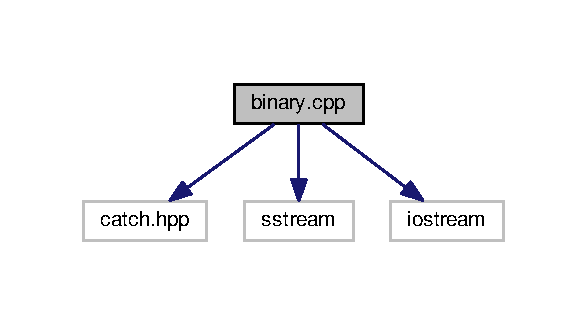
\includegraphics[width=282pt]{binary_8cpp__incl}
\end{center}
\end{figure}
\subsubsection*{Functions}
\begin{DoxyCompactItemize}
\item 
int \hyperlink{binary_8cpp_a961e363a3e72374639e432be6f19c6af}{binary\+\_\+search} (int a\mbox{[}$\,$\mbox{]}, int from, int to, int value)
\item 
\hyperlink{binary_8cpp_a2d4b2d69e71e492dde7fa00d7921087d}{T\+E\+S\+T\+\_\+\+C\+A\+SE} (\char`\"{}Binary Search\char`\"{})
\end{DoxyCompactItemize}


\subsubsection{Function Documentation}
\mbox{\Hypertarget{binary_8cpp_a961e363a3e72374639e432be6f19c6af}\label{binary_8cpp_a961e363a3e72374639e432be6f19c6af}} 
\index{binary.\+cpp@{binary.\+cpp}!binary\+\_\+search@{binary\+\_\+search}}
\index{binary\+\_\+search@{binary\+\_\+search}!binary.\+cpp@{binary.\+cpp}}
\paragraph{\texorpdfstring{binary\+\_\+search()}{binary\_search()}}
{\footnotesize\ttfamily int binary\+\_\+search (\begin{DoxyParamCaption}\item[{int}]{a\mbox{[}$\,$\mbox{]},  }\item[{int}]{from,  }\item[{int}]{to,  }\item[{int}]{value }\end{DoxyParamCaption})}

Finds an element in a sorted array. 
\begin{DoxyParams}{Parameters}
{\em a} & the sorted array with the elements to search \\
\hline
{\em from} & the start of the range to search \\
\hline
{\em to} & the end of the range to search \\
\hline
{\em value} & the value to search for \\
\hline
\end{DoxyParams}
\begin{DoxyReturn}{Returns}
the index of the first match, or -\/1 if not found 
\end{DoxyReturn}


Definition at line 15 of file binary.\+cpp.


\begin{DoxyCode}
16 \{  
17    \textcolor{keywordflow}{if} (from > to) 
18    \{ 
19       \textcolor{keywordflow}{return} -1; 
20    \}
21 
22    \textcolor{keywordtype}{int} mid = (from + to) / 2;
23    \textcolor{keywordflow}{if} (a[mid] == value)
24    \{
25       \textcolor{keywordflow}{return} mid;
26    \}
27    \textcolor{keywordflow}{else} \textcolor{keywordflow}{if} (a[mid] < value)
28    \{
29       \textcolor{keywordflow}{return} \hyperlink{binary_8cpp_a961e363a3e72374639e432be6f19c6af}{binary\_search}(a, mid + 1, to, value);
30    \}
31    \textcolor{keywordflow}{else}
32    \{
33       \textcolor{keywordflow}{return} \hyperlink{binary_8cpp_a961e363a3e72374639e432be6f19c6af}{binary\_search}(a, from, mid - 1, value);
34    \}
35 \}
\end{DoxyCode}
Here is the caller graph for this function\+:\nopagebreak
\begin{figure}[H]
\begin{center}
\leavevmode
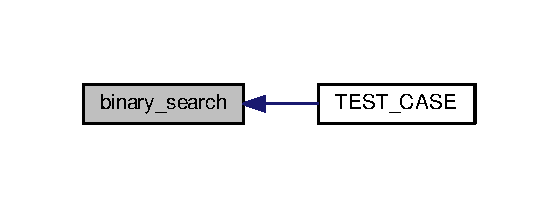
\includegraphics[width=268pt]{binary_8cpp_a961e363a3e72374639e432be6f19c6af_icgraph}
\end{center}
\end{figure}
\mbox{\Hypertarget{binary_8cpp_a2d4b2d69e71e492dde7fa00d7921087d}\label{binary_8cpp_a2d4b2d69e71e492dde7fa00d7921087d}} 
\index{binary.\+cpp@{binary.\+cpp}!T\+E\+S\+T\+\_\+\+C\+A\+SE@{T\+E\+S\+T\+\_\+\+C\+A\+SE}}
\index{T\+E\+S\+T\+\_\+\+C\+A\+SE@{T\+E\+S\+T\+\_\+\+C\+A\+SE}!binary.\+cpp@{binary.\+cpp}}
\paragraph{\texorpdfstring{T\+E\+S\+T\+\_\+\+C\+A\+S\+E()}{TEST\_CASE()}}
{\footnotesize\ttfamily T\+E\+S\+T\+\_\+\+C\+A\+SE (\begin{DoxyParamCaption}\item[{\char`\"{}Binary Search\char`\"{}}]{ }\end{DoxyParamCaption})}



Definition at line 37 of file binary.\+cpp.

Here is the call graph for this function\+:\nopagebreak
\begin{figure}[H]
\begin{center}
\leavevmode
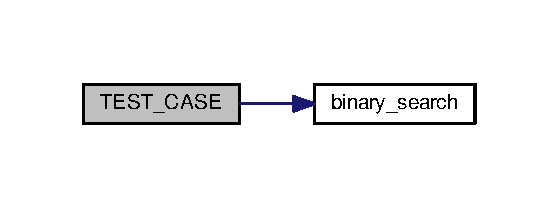
\includegraphics[width=268pt]{binary_8cpp_a2d4b2d69e71e492dde7fa00d7921087d_cgraph}
\end{center}
\end{figure}

\hypertarget{insertion_8cpp}{}\subsection{insertion.\+cpp File Reference}
\label{insertion_8cpp}\index{insertion.\+cpp@{insertion.\+cpp}}
{\ttfamily \#include $<$cstdlib$>$}\newline
{\ttfamily \#include $<$ctime$>$}\newline
{\ttfamily \#include $<$iostream$>$}\newline
{\ttfamily \#include \char`\"{}catch.\+hpp\char`\"{}}\newline
{\ttfamily \#include $<$sstream$>$}\newline
Include dependency graph for insertion.\+cpp\+:\nopagebreak
\begin{figure}[H]
\begin{center}
\leavevmode
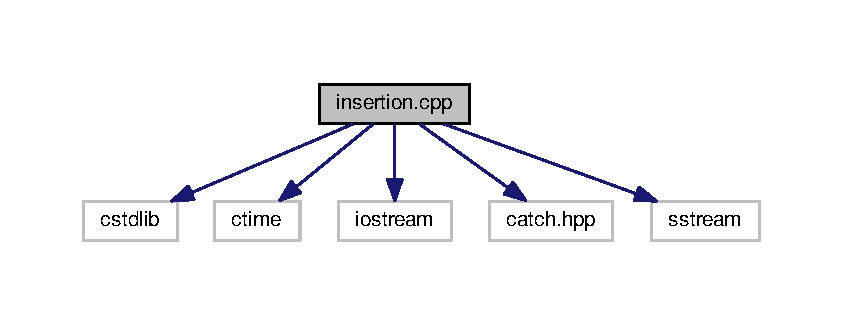
\includegraphics[width=350pt]{insertion_8cpp__incl}
\end{center}
\end{figure}
\subsubsection*{Functions}
\begin{DoxyCompactItemize}
\item 
void \hyperlink{insertion_8cpp_ad43b712bc7e658f7843a1f40f9fb5b09}{insertion\+\_\+sort} (int a\mbox{[}$\,$\mbox{]}, int size)
\item 
void \hyperlink{insertion_8cpp_a5590577c7dd63cd87f70a079fe94d397}{print} (int a\mbox{[}$\,$\mbox{]}, int size)
\item 
\hyperlink{insertion_8cpp_a46b59430c07b056ea10a63cf31a92798}{T\+E\+S\+T\+\_\+\+C\+A\+SE} (\char`\"{}Insertion\char`\"{})
\end{DoxyCompactItemize}


\subsubsection{Detailed Description}
\begin{DoxyRefDesc}{Test}
\item[\hyperlink{test__test000001}{Test}]
\begin{DoxyVerbInclude}
insertion.cpp:68: passed: ss.str() == "83 86 77 15 93 \n15 77 83 86 93 \n" for: "83 86 77 15 93 
15 77 83 86 93 
"
==
"83 86 77 15 93 
15 77 83 86 93 
"
Passed 1 test case with 1 assertion.

\end{DoxyVerbInclude}
 \end{DoxyRefDesc}


\subsubsection{Function Documentation}
\mbox{\Hypertarget{insertion_8cpp_ad43b712bc7e658f7843a1f40f9fb5b09}\label{insertion_8cpp_ad43b712bc7e658f7843a1f40f9fb5b09}} 
\index{insertion.\+cpp@{insertion.\+cpp}!insertion\+\_\+sort@{insertion\+\_\+sort}}
\index{insertion\+\_\+sort@{insertion\+\_\+sort}!insertion.\+cpp@{insertion.\+cpp}}
\paragraph{\texorpdfstring{insertion\+\_\+sort()}{insertion\_sort()}}
{\footnotesize\ttfamily void insertion\+\_\+sort (\begin{DoxyParamCaption}\item[{int}]{a\mbox{[}$\,$\mbox{]},  }\item[{int}]{size }\end{DoxyParamCaption})}

Sorts an array, using insertion sort. 
\begin{DoxyParams}{Parameters}
{\em a} & the array to sort \\
\hline
\end{DoxyParams}


Definition at line 14 of file insertion.\+cpp.


\begin{DoxyCode}
15 \{
16    \textcolor{keywordflow}{for} (\textcolor{keywordtype}{int} i = 1; i < size; i++)
17    \{
18       \textcolor{keywordtype}{int} next = a[i];
19       \textcolor{comment}{// Move all larger elements up}
20       \textcolor{keywordtype}{int} j = i;
21       \textcolor{keywordflow}{while} (j > 0 && a[j - 1] > next)
22       \{
23          a[j] = a[j - 1];
24          j--;
25       \}
26       \textcolor{comment}{// Insert the element}
27       a[j] = next;
28    \}
29 \}
\end{DoxyCode}
Here is the caller graph for this function\+:\nopagebreak
\begin{figure}[H]
\begin{center}
\leavevmode
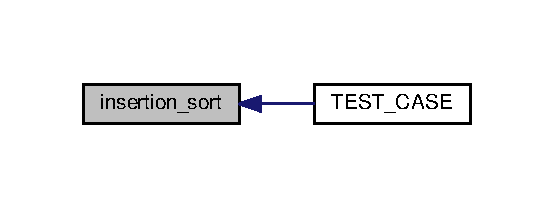
\includegraphics[width=266pt]{insertion_8cpp_ad43b712bc7e658f7843a1f40f9fb5b09_icgraph}
\end{center}
\end{figure}
\mbox{\Hypertarget{insertion_8cpp_a5590577c7dd63cd87f70a079fe94d397}\label{insertion_8cpp_a5590577c7dd63cd87f70a079fe94d397}} 
\index{insertion.\+cpp@{insertion.\+cpp}!print@{print}}
\index{print@{print}!insertion.\+cpp@{insertion.\+cpp}}
\paragraph{\texorpdfstring{print()}{print()}}
{\footnotesize\ttfamily void print (\begin{DoxyParamCaption}\item[{int}]{a\mbox{[}$\,$\mbox{]},  }\item[{int}]{size }\end{DoxyParamCaption})}

Prints all elements in an array. 
\begin{DoxyParams}{Parameters}
{\em a} & the array to print \\
\hline
{\em size} & the number of elements in a \\
\hline
\end{DoxyParams}


Definition at line 36 of file insertion.\+cpp.


\begin{DoxyCode}
37 \{  
38    \textcolor{keywordflow}{for} (\textcolor{keywordtype}{int} i = 0; i < size; i++)
39    \{
40       cout << a[i] << \textcolor{stringliteral}{" "};
41    \}
42    cout << endl;
43 \}
\end{DoxyCode}
Here is the caller graph for this function\+:\nopagebreak
\begin{figure}[H]
\begin{center}
\leavevmode
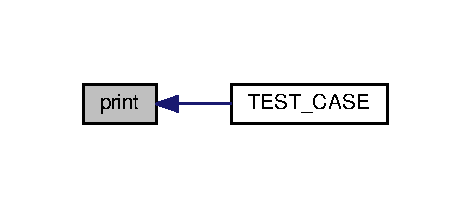
\includegraphics[width=226pt]{insertion_8cpp_a5590577c7dd63cd87f70a079fe94d397_icgraph}
\end{center}
\end{figure}
\mbox{\Hypertarget{insertion_8cpp_a46b59430c07b056ea10a63cf31a92798}\label{insertion_8cpp_a46b59430c07b056ea10a63cf31a92798}} 
\index{insertion.\+cpp@{insertion.\+cpp}!T\+E\+S\+T\+\_\+\+C\+A\+SE@{T\+E\+S\+T\+\_\+\+C\+A\+SE}}
\index{T\+E\+S\+T\+\_\+\+C\+A\+SE@{T\+E\+S\+T\+\_\+\+C\+A\+SE}!insertion.\+cpp@{insertion.\+cpp}}
\paragraph{\texorpdfstring{T\+E\+S\+T\+\_\+\+C\+A\+S\+E()}{TEST\_CASE()}}
{\footnotesize\ttfamily T\+E\+S\+T\+\_\+\+C\+A\+SE (\begin{DoxyParamCaption}\item[{\char`\"{}Insertion\char`\"{}}]{ }\end{DoxyParamCaption})}



Definition at line 51 of file insertion.\+cpp.


\begin{DoxyCode}
52 \{  
53    \textcolor{keyword}{const} \textcolor{keywordtype}{int} SIZE = 5;
54    \textcolor{keywordtype}{int} values[SIZE];
55    \textcolor{keywordflow}{for} (\textcolor{keywordtype}{int} i = 0; i < SIZE; i++)
56    \{
57       values[i] = rand() % 100;
58    \}
59    std::streambuf *b = std::cout.rdbuf(); std::stringstream ss;
60     std::streambuf *sb = ss.rdbuf(); std::cout.rdbuf(sb);
61     \textcolor{comment}{// Now all output will be redirected into ss}
62    \hyperlink{insertion_8cpp_a5590577c7dd63cd87f70a079fe94d397}{print}(values, SIZE);
63    \hyperlink{insertion_8cpp_ad43b712bc7e658f7843a1f40f9fb5b09}{insertion\_sort}(values, SIZE);
64    \hyperlink{insertion_8cpp_a5590577c7dd63cd87f70a079fe94d397}{print}(values, SIZE);
65    \textcolor{comment}{// set output back to the terminal }
66    std::cout.rdbuf(b);
67    
68    CHECK(ss.str() == \textcolor{stringliteral}{"83 86 77 15 93 \(\backslash\)n15 77 83 86 93 \(\backslash\)n"}); 
69    \textcolor{comment}{//return 0;}
70 \}
\end{DoxyCode}
Here is the call graph for this function\+:\nopagebreak
\begin{figure}[H]
\begin{center}
\leavevmode
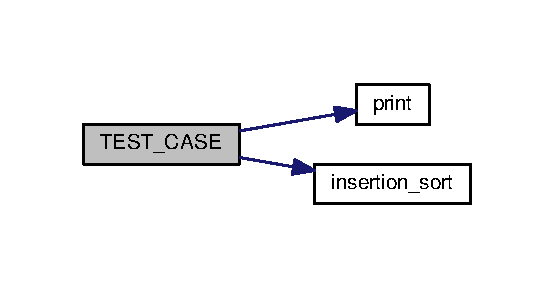
\includegraphics[width=266pt]{insertion_8cpp_a46b59430c07b056ea10a63cf31a92798_cgraph}
\end{center}
\end{figure}

%--- End generated contents ---

% Index
\newpage
\phantomsection
\clearemptydoublepage
\addcontentsline{toc}{section}{Index}
\printindex

\end{document}
